\documentclass[a4paper]{article}

%###############################################################
%###############################################################
%##### This template is based on EngrXiv preprint template #####
%###############################################################
%###############################################################

%% Language and font encodings
\usepackage[T1]{fontenc}
\usepackage[utf8x]{inputenc}
\usepackage[english]{babel}

\usepackage[colorlinks=true, allcolors=blue]{hyperref}

\urlstyle{tt}
\newcommand{\email}[1]{\href{mailto:#1}{\tt{\nolinkurl{#1}}}}
\newcommand{\orcid}[1]{ORCID: \href{https://orcid.org/#1}{\tt{\nolinkurl{#1}}}}

\usepackage[sfdefault,lf]{carlito}
%% The 'lf' option for lining figures
%% The 'sfdefault' option to make the base font sans serif
\usepackage[parfill]{parskip}
\usepackage{float}
\renewcommand*\oldstylenums[1]{\carlitoOsF #1}
\usepackage{fancyhdr}
\usepackage{natbib}
\usepackage{authblk}
\setlength{\headheight}{41pt}

%% Sets page size and margins
\usepackage[a4paper,top=3cm,bottom=2cm,left=3cm,right=3cm,marginparwidth=1.75cm]{geometry}

%% Useful packages
\usepackage{amsmath}
\usepackage{graphicx}
\usepackage{booktabs}

\usepackage[colorinlistoftodos]{todonotes}

%\renewcommand{\headrulewidth}{0pt}
\fancyhead[L]{Posted: \today}
\fancyhead[R]{

\includegraphics[width=4cm]{inarxiv_logo.png}
}
\pagestyle{plain}
\title{Membangun Repositori Institusional (Bagian 1)}
\author[1,*]{Dasapta Erwin Irawan}
\author[2]{Sparisoma Viridi}
\author[3]{Eueung Mulyana}
%\author[2,+]{Derek Author}
\affil[1]{Fakultas Ilmu dan Teknologi Kebumian ITB; \orcid{0000-0000-0000-0000}}
\affil[2]{Fakultas Matematika dan Ilmu Pengetahuan Alam ITB; \orcid{0000-0000-0000-0000}}
\affil[3]{Sekolah Teknik Elektro dan Informatika ITB; \orcid{0000-0000-0000-0000}}
\affil[+]{these authors contributed equally to this work}
\affil[*]{Corresponding author: \email{dasaptaerwin@gmail.com}}
\date{}

\begin{document}
\maketitle
\thispagestyle{fancy}

\begin{abstract}
Dokumen ini merupakan hasil komunikasi intensif antara kedua penulis melalui surel dan WA pada periode April-Juni 2017.

Berikut ini adalah dokumen awal panduan pembangunan Repositori Institusional (RI). RI sangat diperlukan sebagai bentuk \textit{rapid dissemination }hasil riset institusi, karena publikasi formal seringkali tidak tersedia segera setelah riset selesai dilakukan. Materi yang diunggah ke RI adalah berbagai output riset dari "hulu" ke "hilir", dari data, lembar kerja (\textit{working papers}), hingga makalah dalam versi \textit{pre} atau \textit{post print}.

Dalam implementasinya RI akan memerlukan kerjasama yang baik antara penulis/peneliti (terdiri dari dosen/peneliti/mahasiswa) sebagai pelaksana, staf perpustakaan (sebagai \textit{data kurator} dan \textit{data regulator}), serta Kantor Wakil Rektor Bidang Riset, Inovasi, dan Kemitraan (WRRIM) sebagai koordinator.

Beberapa komponen yang perlu mendapatkan perhatian adalah: piranti keras/infrastruktur terdiri dari ketersediaan server dan jaringan, piranti lunak terdiri dari RI \textit{interface}, \textit{research data management policy}), dan sumber daya manusia meliputi pendidikan staff (di tingkat perpustakaan), dosen, peneliti, serta mahasiswa.

Pertama yang perlu dibangun adalah awareness tentang research management secara umum, \textit{research documentation }dan \textit{self-archiving}, serta \textit{rapid dissemination}.

Membangun infrastuktur dan sistem RI adalah satu hal berat, tapi hal yang paling berat adalah menumbuhkan kesadaran sivitas akademik ITB untuk melakukan \textit{self-archiving } dan berbagi informasi dimulai dari tingkat dosen hingga mahasiswa.

Keywords: repository institutional, open access, rapid dissemination

\end{abstract}

\section{Pendahuluan}
%########################################
\subsection{Latar belakang}
%########################################

Kebutuhan akan repositori institusional (RI) disebabkan beberapa hal sebagai berikut (\href{https://www.slideshare.net/smtch/institutional-repositories-16233657}{IR review}):

\begin{itemize}
\item Riset berkembang pesat tetapi kapasitas akademia (dosen, peneliti, mahasiswa) belum mampu mengikutinya dengan jumlah publikasi yang seimbang,
\item Masalah ke-1 sering dihubungkan dengan tuntutan dari pemerintah (melalui Kemristekdikti) mengenai publikasi internasional (dalam Bahasa Inggris) yang bukan merupakan \textbf{bahasa ibu}, serta ketentuan tentang media jurnal yang diakui bereputasi (yang mana antrian publikasi akan semakin panjang),
\item Masalah ke-2 ditambah dengan proses \textit{peer review} menyebabkan publikasi baru terbit dalam waktu yang cukup lama. 
\end{itemize}

Dengan adanya kendala utama di atas, maka hasil riset makin tidak tersampaikan kepada masyarakat. Kalaupun akan tersampaikan, maka akan perlu waktu yang cukup lama. Untuk menjamin agar hasil riset sampai kepada target penggunanya, peneliti memerlukan stamina yang stabil sepnjang periode itu. RI diharapkan mengisi kekosongan ruang dan waktu ini, yakni sebagai "media penghubung" antara peneliti dan masyarakat secara lebih instan tanpa batasan-batasan Pihak ke-3. 

RI yang diperlukan adalah dengan karakter sebagai berikut:

\begin{enumerate}
\item \textbf{bebas}: RI bebas digunakan oleh dosen, asisten peneliti, mahasiswa (program sarjana/magister/doktor).
\item \textbf{termoderasi}: RI yang memiliki Tim Pengelola yang handal untuk memoderasi.
\item \textbf{terkendali}: RI yang memiliki sistem otorisasi handal yang memungkinkan tiga pihak: penulis, Dekan Fakultas/Sekolah, dan LPPM untuk mengendalikan lingkup pembagian pranala dokumen.
\item \textbf{terbuka}: RI yang terbuka, sehingga dapat ditemukan oleh Mesin Pencari dengan mudah, seperti diindeks oleh \href{scholar.google.com}{Google Scholar}. Untuk menambah potensi keterbacaan (\textit{readability}), seperti:

    \begin{itemize}
    \item Directory of Open Access Repository (\href{http://www.opendoar.org/}{DOAR}) dengan menambahkan repositori ITB ke dalam basis datanya (\href{http://www.opendoar.org/suggest.php}{tautan}),
    \item \href{http://datacite.org}{Data Cite}, dan 
    \item \href{https://www.ncbi.nlm.nih.gov/pmc/}{Pubmed Central}.
    \end{itemize}

\item \textbf{Aman}: RI yang menjamin keamanan akses. Pengguna tidak dapat mengakses data melebihi yang seharusnya. 

\item \textbf{Berkelanjutan}: RI yang menjamin preservasi data dalam waktu yang lama. Lamanya durasi penyimpanan ini masih memerlukan kajian lebih lanjut.

\item \textit{\textbf{Reproducible}}: RI dengan menawarkan fitur yang mendukung penyimpanan material riset, sehingga dapat direproduksi (\textit{reproducible}) dengan mudah. Salah satunya adalah menyediakan struktur folder berisi data, kode analisis, dan hasil analisis.

\item \textbf{\textit{Version control} dan \textit{forking}}: RI yang memiliki fitur untuk mendokumentasikan berbagai versi dokumen (\textit{version control} atau kendali versi) dan penggandaan dokumen (\textit{forking}) atau proyek. Salah satu yang mempopulerkan istilah ini, \textit{forking}, adalah situs jejaring pemrogram \href{http://github.com}{GitHub}.  
% * <d_erwin_irawan@yahoo.com> 2017-12-20T14:58:58.898Z:
% 
% > Salah satu yang mempopulerkan istilah ini, \textit{forking}, adalah situs jejaring pemrogram \href{http://github.com}{GitHub}. Apakah benar?
% ^.

\end{enumerate}
Dunia telah mengenal repositori dan RI cukup lama. Beberapa hasil kajian awal adalah sebagai berikut. Kondisi RI di dunia menurut \href{https://dataverse.org/}{Dataverse Project} (Gambar \ref{RI_location}). Di Indonesia ada RI milik \href{http://www.cofor.org}{CIFOR} (Center for International Forestry Research) yang berdomisili di Bogor.

\begin{figure}[!ht]
  \centering
  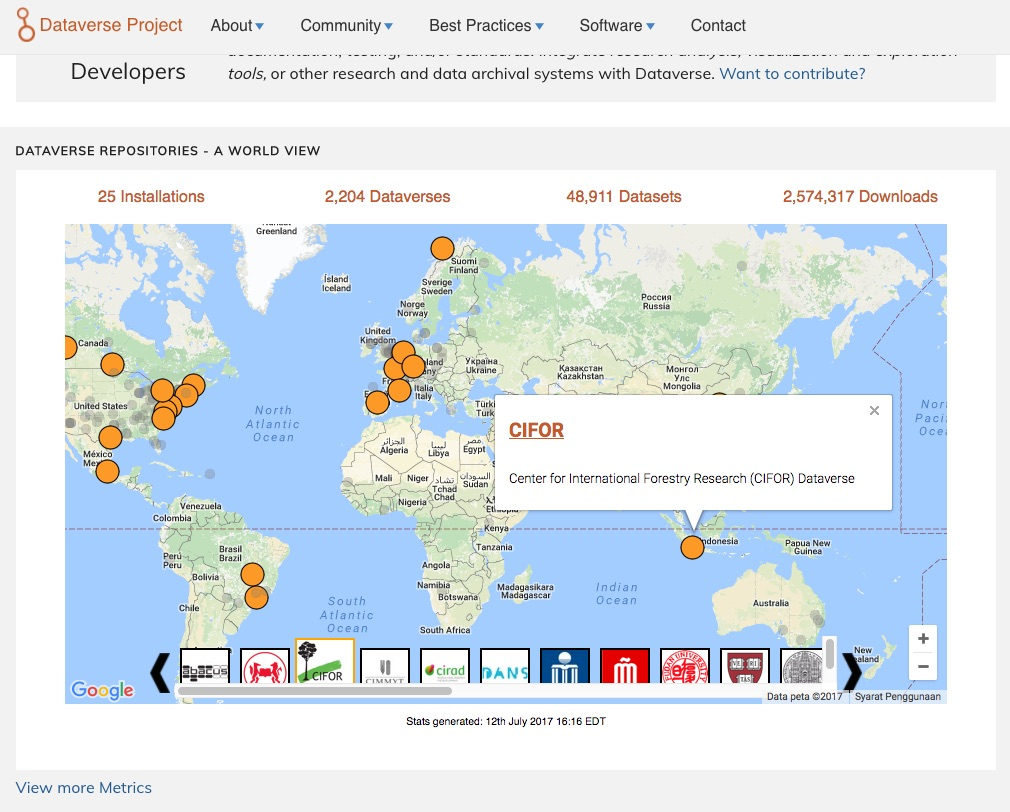
\includegraphics[width=1\textwidth]{GS4.jpg}
  \caption{Posisi RI dengan piranti lunak Dataverse}
  \label{RI_location}
\end{figure}

Dengan jumlah dokumen yang diunggah dan diunduh seperti pada Gambar \ref{up_downloads}.

\begin{figure}[!ht]
  \centering
  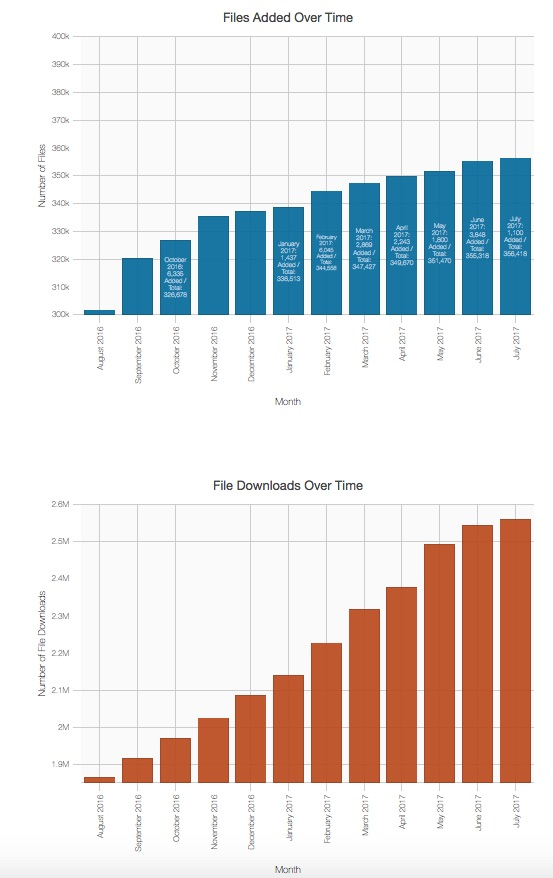
\includegraphics[width=0.8\textwidth]{GS5.jpg}
  \caption{Jumlah dokumen yang diunggah dan diunduh}
  \label{up_downloads}
\end{figure}

Dengan jumlah dokumen yang diunggah berdasarkan bidang ilmu seperti pada Gambar \ref{kategori}.

\begin{figure}[h!]
  \centering
  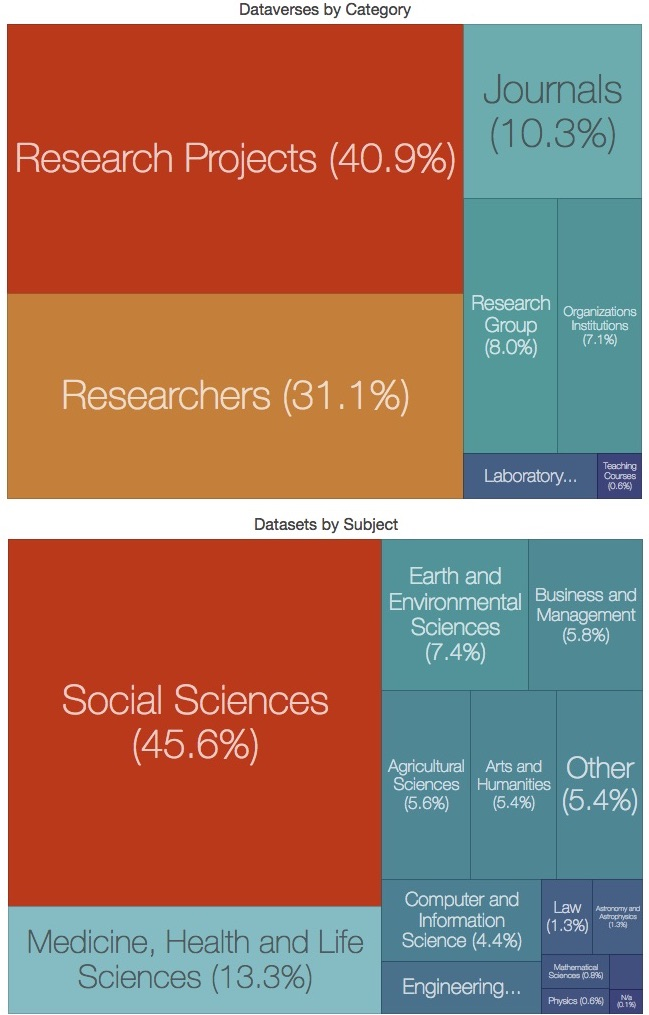
\includegraphics[width=0.8\textwidth]{GS6.jpg}
  \caption{Dokumen yang diunggah berdasarkan kategori dan bidang ilmu}
  \label{kategori}
\end{figure}

Statistik di atas didapatkan dari \href{https://dataverse.org/metrics}
{Dataverse Project Metric} baru untuk RI yang menggunakan piranti lunak \textit{Dataverse}. Data lainnya, bisa didapatkan dari \href{http://roar.eprints.org/}{R-ROAR} (Registry of Open Access Repositories), yang menyatakan ada 111 RI \textit{open access }di Indonesia. Beberapa diantaranya: \href{http://eprints.lib.ui.ac.id/}{UI-ana}, \href{http://repository.umm.ac.id/}{UMM}, dan {http://eprints.binus.ac.id/}{Binus}, \href{http://eprints.upnjatim.ac.id/}{UPN Jatim}, \href{http://eprints.sunan-ampel.ac.id/}{IAIN SUnan Ampel, Surabaya}. Seluruhnya menggunakan piranti lunak \href{http://eprints.org}{e-Prints} 

\subsection{Isu yang akan berkaitan dengan RI}
%########################################

Berikut ini adalah beberapa isu internasional yang akan berkaitan dengan RI. Tanggungjawab pengembang/pengelola untuk dapat mensosialisasikannya kepada sivitas akademik ITB.

\begin{enumerate}
\item \href{http://osc.universityofcalifornia.edu/2016/09/who-owns-your-data/}{Siapa yang memiliki data (who owns your data)} adalah isu yang mengemuka beberapa tahun terakhir. Setelah data dikumpulkan, terutama oleh institusi pendidikan, pemerintahan, atau lembaga nir-laba, lantas siapakah pemilik data tersebut,

\item Harvard University telah merilis praktek yang baik dalam mengelola data \href{https://dataverse.org/best-practices/harvard-dataverse-general-terms-use}{Harvard Dataverse Project},

\item Apakah data \textit{replication}, \textit{re-use} dan \textit{re-mix} strategis untuk perguruan tinggi di negara berkembang? Beberapa dokumen berikut ini menunjukkan hal tersebut: \href{http://www.openoasis.org/index.php?option=com_content&view=article&id=28:developing-countries&Itemid=253}{Open Access and Developing Countries}, \href{https://www.coar-repositories.org/files/Open-Access-Asia-Report.pdf}{Asian Open Access Meeting
Report}, dan \href{https://www.weforum.org/agenda/2015/08/why-open-access-to-information-is-crucial-for-developing-countries/}{Why open access to information is crucial for developing countries}, juga pengembangan \href{http://www.projecttier.org/}{Project TIER (Teaching Integrity Empirical Research)}.

\item Apakah RI strategis untuk mendukung misi dan visi ITB? Beberapa dokumen berikut ini adalah beberapa rujukan yang dapat digunakan: \href{http://www.emeraldinsight.com/doi/abs/10.1108/OCLC-04-2014-0022}{The role of institutional repositories in developing the communication of scholarly research}, \href{http://citeseerx.ist.psu.edu/viewdoc/download?doi=10.1.1.474.8441&rep=rep1&type=pdf}{Case studies on institutional repository development: Creating narratives for project management and assessment},

\item Apakah RI memiliki potensi masalah? Berikut ini rujukan yang dapat digunakan: \href{http://www.dlib.org/dlib/may07/henty/05henty.html}{Ten Major Issues in Providing a Repository Service in Australian Universities}, \href{http://www.ijodls.in/uploads/3/6/0/3/3603729/vol-2_issue-4_1-16.pdf}{An investigation to the challenges of institutional repositories development in six academic institutions in Nigeria},
\href{http://cameronneylon.net/blog/the-trouble-with-institutional-repositories/}{The trouble with institutional repositories}

\item Bagaimana kesiapan insfrastruktur RI? Salah satu yang perlu dipertimbangkan adalah infrastruktur piranti lunak, seperti dijelaskan dalam dokumen ini \href{https://open.library.ubc.ca/cIRcle/collections/graduateresearch/42591/items/1.0075768}{Komparasi piranti lunak RI oleh University of  British Columbia}

\end{enumerate}

\subsection{Definisi RI}
%########################################

Beberapa definisi RI:

\begin{quotation} 
An institutional repository is an archive for collecting, preserving, and disseminating digital copies of the intellectual output of an institution, particularly a research institution (\href{https://en.wikipedia.org/wiki/Institutional_repository}{Wikipedia}) 
\end{quotation} 

\begin{quotation} a university-based institutional repository is a set of services that a university offers to the members of its community for the management and dissemination of digital materials created by the institution and its community members. It is most essentially an organizational commitment to the stewardship of these digital materials, including long-term preservation where appropriate, as well as organization and access or distribution (\href{https://blogs.libraries.indiana.edu/scholcomm/2011/08/23/2-what-is-an-institutional-repository/}{Indiana University Library}). 
\end{quotation}

\begin{quotation}
Unlike some disciplinary repositories, institutional repositories contain research by an institution's researchers in many different disciplines. By offering unrestricted access, institutional repositories offer the widest possible sharing of faculty research (\href{http://guides.library.jhu.edu/c.php?g=202599&p=1335149}{Johns Hopkins Sheridan Libraries}). 
\end{quotation}

\subsection{Benefit RI}
%################################################

Benefit RI adalah sebagai berikut: 

\begin{itemize}
\item meningkatkan diseminasi hasil riset secara cepat dalam skala global: karena semua material diunggah daring, sehingga dapat diakses oleh siapapun dan dari manapun, 

\item dengan menggunakan indexing Google Scholar (salah satunya), maka dapat meningkatkan keterbacaan (\textit{readability}) dokumen,

\item menghindari pencurian ide (\textit{scooping}) atau plagiarisme, karena setiap dokumen akan muncul dalam pencarian Google maupun Google Scholar,

\item tautan yang permanen (permanent link/url) serta 

\item pengarsipan jangka panjang yang aman (\textit{safe long-term archiving}). 
\end{itemize}

Benefit yang \textit{intangible} adalah:

\begin{itemize}
\item meningkatkan kepercayaan diri mahasiswa dan peneliti pemula (\textit{early career researcher}/ECR), karena telah melihat dokumennya tertayang secara terbuka dan dapat diakses oleh siapapun yang memerlukan, dari mana pun,

\item bila para pengunggah (dosen, peneliti, mahasiswa) memiliki akun profil \href{orcid.org}{ORCID}, maka materi yang diunggah dapat masuk secara otomatis ke profil ORCID (hubungan \textit{auto-sync}).
\end{itemize}

Beberapa benefit di atas tidak mengurangi makna dokumen publikasi yang telah melalui proses \textit{peer-review}. Namun demikian, dengan asumsi bahwa berbagai dokumen dalam RI adalah dokumen yang saintifik, serta telah memiliki tautan permanen (bahkan DOI), maka dokumen-dokumen tersebut dapat disitasi dalam dokumen secara formal. 

\section{Sekilas pengujian cepat beberapa repositori} 
%################################################

Kami telah mengadakan pengujian singkat tentang repositori untuk menguji keterbacaannya secara daring. Google Scholar kami gunakan dalam pengujian. Kata kunci di bidang geologi kami gunakan, "geologi dan hidrogeologi". Kata kunci tersebut biasa digunakan sebagai judul skripsi mahasiswa geologi. Harapannya pencarian akan memunculkan dokumen skripsi geologi yang tersimpan di repositori suatu universitas.

\subsection{Hasil sementara}
%################################################

Pencarian dengan kata kunci "geologi dan hidrogeologi" menghasilkan halaman pertama berisi 10 dokumen. Enam dokumen tercatat disimpan di repositori Universitas Petra, UGM, Unisba, IPB, dan Unpad .
% * <d_erwin_irawan@yahoo.com> 2017-12-20T15:39:05.569Z: insert link to each RI
% ^ <d_erwin_irawan@yahoo.com> 2017-12-20T15:39:23.564Z.

\begin{figure}[h!]
  \centering
  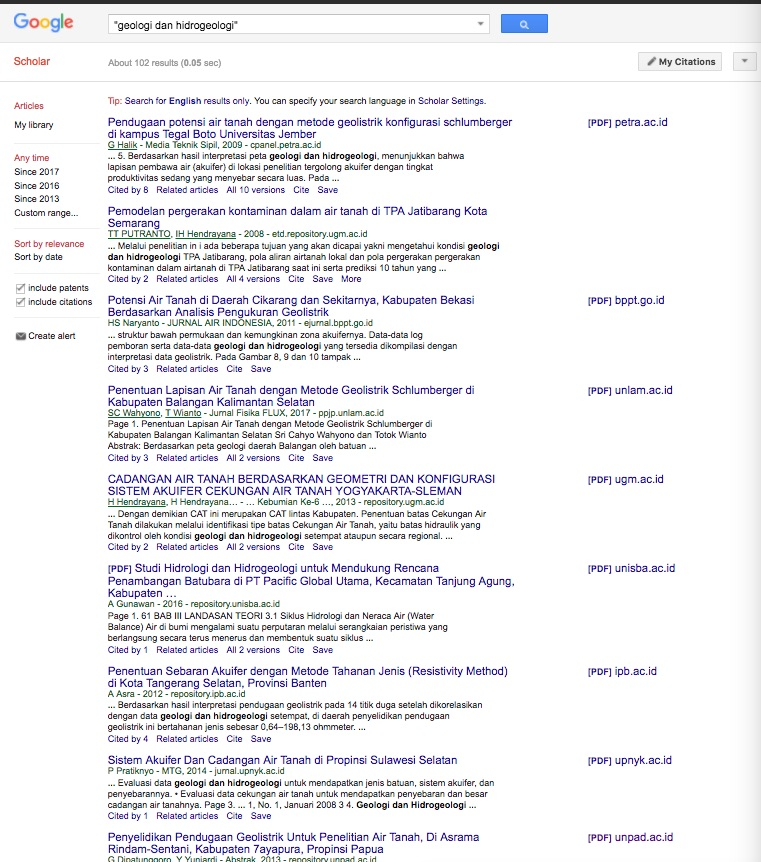
\includegraphics[width=0.5\textwidth]{GS1.jpg}
  \caption{Hasil pencarian di laman Google Scholar dengan kata kunci "geologi dan hidrogeologi"}
\end{figure}

Kemudian kami coba mengakses dokumen berjudul: 
\begin{itemize}
\item "Cadangan air tanah berdasarkan geometri dan konfigurasi sistem akuifer Cekungan Air Tanah Yogyakarta-Sleman". Dokumen terbuka dengan sempurna  
\item "Penyelidikan Pendugaan Geolistrik Untuk Penelitian Air Tanah, Di Asrama Rindam-Sentani, Kabupaten Jayapura, Propinsi Papua". Dokumen terbuka dengan sempurna.

\end{itemize}

Dari hasil pencarian tersebut dapat dilihat bahwa ITB tidak muncul, padahal di laman \href{http://digilib.itb.ac.id}{Digital Library ITB} delapan dokumen skripsi tercatat menggunakan judul tersebut.

\begin{figure}[h!]
  \centering
  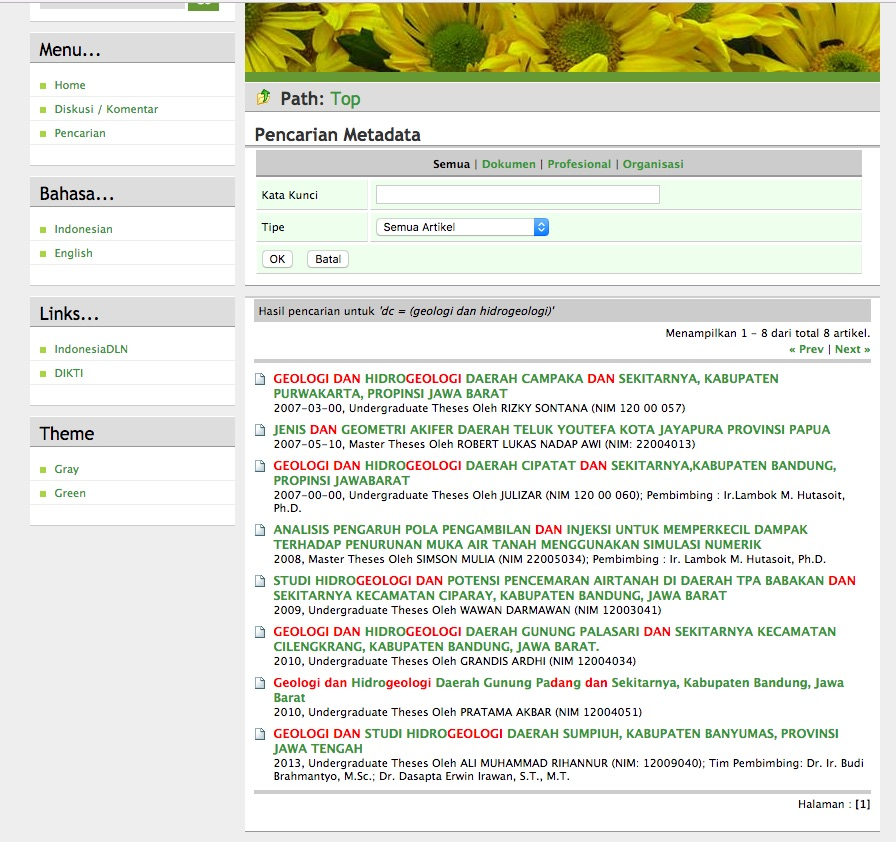
\includegraphics[width=0.5\textwidth]{GS2.jpg}
  \caption{Hasil pencarian di laman Digital Library dengan kata kunci "geologi dan hidrogeologi"}
\end{figure}

Dalam hal ini ada beberapa pertanyaan yang perlu dijawab:

\begin{itemize}
\item Bagaimana Unpad, UGM, Unisba, Unika Petra dapat memunculkan karyanya dalam hasil pencarian? Apakah piranti lunak dan sistem mereka mendukung untuk itu?
\item Dari satu sisi Digilib ITB memang sebuah repositori tetapi tidak "terbuka". Apakah hal ini bisa diubah? 
\item 
\end{itemize}

Pengecekan lebih lanjut ke Repositori Unpad telah dilakukan. Kami menemukan bahwa repositori menggunakan piranti lunak \href{http://www.eprints.org/uk/}{E-Prints} yang gratis dan terbuka (\textit{open source}). Namun demikian data dokumen pada beberapa tahun tidak dapat dibuka.

\begin{figure}[h!]
  \centering
  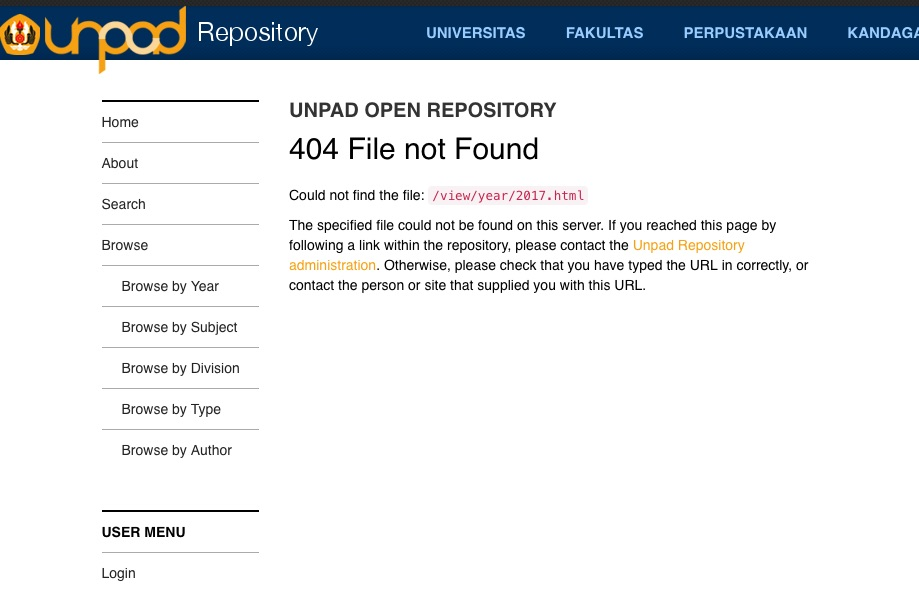
\includegraphics[width=1\textwidth]{GS3.jpg}
  \caption{Tangkapan layar Reporsitori Unpad}
\end{figure}

\section{Beberapa hal teknis tentang RI}
%##############################
\subsection{Isi}
%################################################

RI dapat berisi beberapa dokumen akademik berikut ini \citep{rinehart_breaking_2017}:

\begin{enumerate}
\item kertas kerja (\textit{working papers}): sebuah makalah yang menjelaskan riset yang sedang berjalan, bisa diartikan juga sebagai catatan riset, 

\item laporan teknis (\textit{technical reports}): laporan riset yang telah selesai dan lengkap. Laporan di sini dapat diartikan sebagai laporan riset, pengabdian kepada masyarakat, juga layanan kepakaran.

\item slide presentasi (\textit{conference slides}): slide paparan presentasi dalam format ppt, odp, maupun pdf,

\item prosiding \textit{proceedings}: kumpulan makalah atau abstrak hasil seminar. Dokumen dapat diunggah oleh panitia seminar atau peserta.

\item \textit{preprints} dan \textit{postprints}: makalah versi sebelum \textit{peer review} dan versi setelah \textit{peer review}. Untuk dokumen jenis ini perlu sosialisasi lebih luas ke para pengelola jurnal dalam negeri agar tidak dikategorikan duplikasi. Pengelola jurnal luar negeri dalam kasus ini lebih paham. Kebijakannya dapat diperiksa dalam direktori \href{http://www.sherpa.ac.uk/romeo/index.php}{Sherpa/Romeo}. 

\item \textit{datasets}: data hasil riset, termasuk di dalamnya skripsi, tesis, dan disertasi. Data dalam hal ini akan diposisikan sebagai output riset yang independen, dilengkapi dengan lisensi terpisah. Dokumen laporan (skripsi, tesis, disertasi) akan menyitat data ini. 

\item materi multimedia, mencakup: video perkuliahan, rekaman suara (\textit{podcasts}), rekaman layar komputer (\textit{screencasts}), animasi.

\item bahan ajar: ada perdebatan di sini, yakni apakah bahan ajar adalah milik dosen pengampu (penyusun bahan ajar) atau perguruan tinggi, karena bahan ajar tersebut termasuk di dalam dokumen kurikulum perguruan tinggi. Mayoritas perguruan tinggi belum pernah membuat kesepakatan ini dengan para dosennya. Bila bahan ajar milik perguruan tinggi, maka bisa jadi bahan tersebut tidak dapat masuk ke dalam RI atau masuk ke dalam RI tapi dengan pengaturan hak akses terbatas (hanya para pihak yang terlibat dalam proses belajar mengajar. Tetapi bila bahan ajar tetap menjadi milik dosen pengampu, maka dosen berhak untuk memuatnya di berbagai media, termasuk RI.

\item skripsi, tesis, disertasi: untuk jenis dokumen ini, juga masih menjadi perbincangan. Apakah dengan mengunggah dokumen ini akan meningkatkan plagiarisme, karena dokumen menjadi mudah untuk diunduh pihak luar. Di sisi lain, pengelola perguruan tinggi juga khawatir bahwa dokumen lulusannya terdeteksi mengandung plagiarisme. Proses pembimbingan di banyak perguruan tinggi tidak termasuk pemeriksaan kesamaan (\textit{similarity checker}). Untuk mengatasinya beberapa perguruan tinggi mengunggah versi abstrak panjang dari tesis.   

\item dokumen kegiatan mahasiswa lainnya: dapat berupa laporan kegiatan pengabdian kepada masyarakat, makalah kompetisi, ide proposal kegiatan, dll.

\end{enumerate}

\subsection{Karakter dokumen dalam RI}
%################################################

Karakter dokumen yang diharapkan:

\begin{enumerate}
\item \textbf{lengkap}: dokumen bersifat lengkap dan tidak terpotong-potong.

\item \textbf{terintegrasi}: ada tautan yang jelas antara dokumen utama dengan data mentah, serta lampiran-lampirannya yang diunggah secara terpisah. Dalam hal ini dikenalkan konsep bahwa data, foto, gambar, adalah output riset yang terpisah dan dapat disitasi dalam dokumen lengkap.

\item \textbf{memuat data mentah}: data yang diunggah adalah data mentah dalam format yang kompatibel dengan berbagai aplikasi, misal csv, txt. Bila format binary seperti xls, xlsx disetujui untuk digunakan, maka perlu ditetapkan versinya. Tabel data tidak dalam format pdf untuk memudahkan re-analisis oleh pengguna.

\item \textbf{resolusi tinggi}: bila data yang diunggah berupa foto atau gambar, maka diharapkan obyek tersebut beresolusi tinggi,

\item \textbf{bersifat \textit{searchable}}: proses pencarian kata, angka, atau obyek lain dimungkinkan di dalam dokumen yang diunggah. Ini hanya memungkinkan bila dokumen tidak dapat format pdf yang diproteksi, format html atau xml akan lebih baik. Bila format pdf yang digunakan. Untuk itu, skema metadata (\textit{metadata schema}) perlu disusun dengan rapih dan sistematis.

\end{enumerate}

\section{Peta jalan (\textit{Roadmap})}

\subsection{Beberapa panduan}
Berikut ini adalah komponen RI dan bagaimana mencapainya %insert comment from Gene Usyd mengenai ontology, vocab, metadata schema, etc

Contoh alur kerja RI dan hubungan antar unit kerja, yang terdiri dari unit pendidikan, unit penelitian dan pengabdian kepada masyarakat, unit layanan kepakaran, dan pribadi dosen.

\begin{figure}[h!]
  \centering
  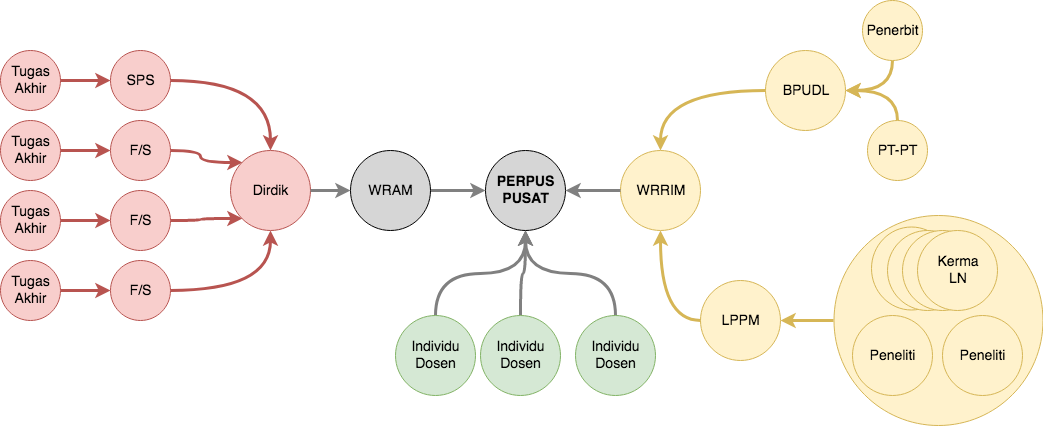
\includegraphics[width=1\textwidth]{RI.png}
  \caption{Rantai proses sebuah RI} 
\end{figure}

\subsection{Peta jalan di tingkat perguruan tinggi}
Berikut ini adalah usulan roadmap pembangunan RI di tingkat perguruan tinggi.
\\
%insert roadmap


\begin{figure}[h!]
  \centering
  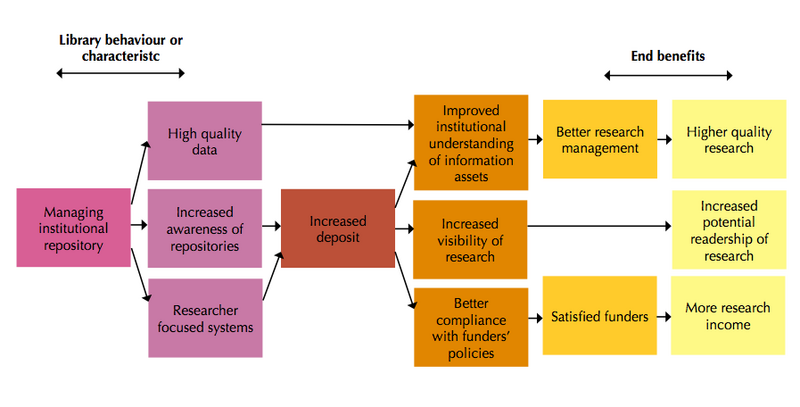
\includegraphics[width=1\textwidth]{IR_chain.png}
  \caption{Rantai proses sebuah RI (\href{http://hlwiki.slais.ubc.ca/index.php/Institutional_repositories}{IR Canada})}
\end{figure}

%\begin{figure}[h!]
%  \centering
%  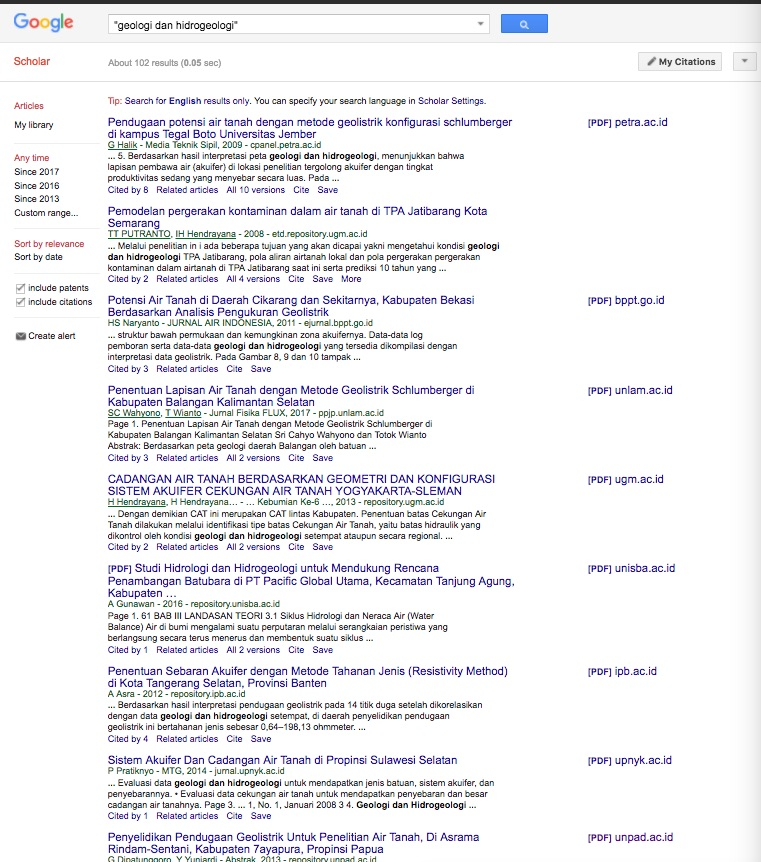
\includegraphics[width=0.5\textwidth]{GS1.jpg}
%  \caption{Hasil pencarian di laman Google Scholar dengan kata kunci "geologi dan hidrogeologi"}
%\end{figure}

%################################################
\section{Beberapa hal yang perlu diputuskan}
%################################################

Berikut ini adalah beberapa hal yang perlu dipikirkan dan diputuskan di tingkat perguruan tinggi sebelum membangun sebuah RI (\href{https://uh-ir.tdl.org/uh-ir/bitstream/handle/10657/1623/DsstFinalReport.pdf}{DIGITAL SCHOLARSHIP ROAD MAP}):

\begin{enumerate}

\item \textbf{Akses}: akses apakah berlaku umum secara bebas, ataukah berjenjang.

% Note: Sebagai catatan, di ITB telah lama ada \href{digilib.itb.ac.id}{Digital Library} berisi dokumen skripsi, tesis, dan disertasi mahasiswa. Diusulkan agar ada pemisahan antara dokumen lama dan baru. Dokumen lama yang telah diunggah ke Digilib tidak perlu diganggu. Hanya dokumen baru saja yang perlu diunggah ke RI. \textbf{Kesimpulan sementara}: Sementara ini Digilib akan tetap seperti sekarang bersifat tertutup, karena kekhawatiran terhadap kualitas penulisan tesis (misal: plagiarisme). Hal ini karena tugas dosen pembimbing tidak sampai ke pengecekan hal tersebut. 

\item \textbf{Dokumen yang boleh diunggah}: sesuai dengan daftar di atas, jenis dokumen perlu untuk disepakati. Dokumen yang potensial adalah: tugas akhir (skripsi, tesis, disertasi), laporan kegiatan (riset, pengabdian kepada masyarakat, layanan kepakaran), protokol analisis data, \textit{preprint}/\textit{postprint}.  

\item \textbf{Pengunggah dokumen}: Apakah pemrosesan dan pengunggahan dokumen menjadi tanggungjawab pustakawan ataukah peneliti/penulis secara langsung.

% Note: Saat ini belum ada staf khusus, staf perpus terbatas. SK tentang kewajiban serah-simpan telah terbit.

% Pengunggah berjenjang: peneliti (skripsi/tesis/disertasi) - bisa mahasiswa atau pembimbingnya, LPPM (dokumen layanan kepakaran di bawah SPK), peneliti utama atau principal investigator (riset dan PKM). Keduanya perlu memperhatikan perjanjian atau kontrak yang telah ada. 

\item \textbf{Pengelolaan RI}: apakah perguruan tinggi akan mengelola server RI sendiri atau bekerjasama dengan pihak ke-3, perusahaan \textit{not for profit}, misal \href{osf.io}{Open Science Framework}, \href{zenodo.org}{Zenodo} contoh \href{https://zenodo.org/communities/itbopendatarepo/}{ITB initiative of open repository}, \href{Figshare.com}{Figshare} contoh \href{https://figshare.com/authors/Dasapta_Erwin_Irawan/762036}{Dasapta Erwin Irawan repository}, atau jejaring \href{https://dataverse.org/}{Data Verse} contoh \href{https://dataverse.harvard.edu/}{Harvard Data Verse}. 

% Note: ITB akan mengelola RI sendiri dengan menggunakan piranti lunak open source Eprints, didukung dengan layanan data repositori dan preprint server berbasis OSF.

\item \textbf{Infrastruktur}: jaringan dan media penyimpanan, mengingat data atau dokumen yang diunggah berukuran besar.

\item \textbf{Sosialisasinya}: Mengingat hal-hal seperti ini bila salah dalam penyampaian akan berakibat dosen merasa bertambah pekerjaannya. 

% Note: ITB dapat menyebarkan minat melalui kuesioner, perlu diseminasi kontinyu 

\item Dokumen \textit{Research Data Management} (RDM) yang belum disusun. Kita dapat merujuk kepada beberapa dokumen: Havard Dataverse RDM (Usyd library RDM). % <<Note: add Gene explanation>>.

Minimum metadata (from Gene):
\begin{enumerate}

\item Identifier*: unique code used to identify dataset, eg. DOI
\item Creator*             
\item Title*
\item Publisher*
\item Publication Year*
\item Subject
\item Contributor
\item Date
\item Language
\item Resource Type* uses a simple vocabulary: Audiovisual, Collection, Data Paper, Dataset, Event, Image, Interactive Resource, Model, Physical Object, Service, Software, Sound, Text, Workflow, Other
\item Alternate Identifier: eg. handle if primary identifier is a DOI
\item Related Identifier: eg. DOI of journal article based on dataset
\item Size
\item Format
\item Version
\item Rights/license:eg. CC-BY license
\item Description
\item GeoLocation
\item Funding Reference

\end{enumerate}

\item Dokumen \textit{copyright transfer agreement }(CTA) atau \textit{Submission Agreement }(SA) yang belum disusun. Dokumen ini bisa berlaku dua arah, dari perguruan tinggi mentransfer hak ke pihak lain (sivitas ITB atau di luar ITB), atau dari penulis/penyusun (bisa dosen atau mahasiswa) ke perguruan tinggi. 

% <<Note: Dokumen ini bisa berlaku dua arah, dari ITB mentransfer hak ke pihak lain (sivitas ITB atau di luar ITB), atau dari penulis/penyusun (bisa dosen atau mahasiswa) ke ITB.>> 

% <<Note: Referensi yang bisa digunakan: CTA Universiti Malaya, xxx, xxx. Bila terjadi transfer hak cipta, maka dokumen CTA ini dapat menyatu dengan berbagai dokumen di bawah ini>>

\begin{enumerate}
\item berbagai dokumen riset skripsi/tesis/mahasiswa, 
\item laporan riset bekerjasama dengan pihak ke-3 (misal Kemristekdikti, Osaka Gas, Asahi Glass, dll),
\item laporan layanan kepakaran yang bekerjasama dengan pihak ke-3,
\item karya seni,
\item etc 
\end{enumerate}

\item Ontology, vocabulary, metadata schema: tiga komponen penting ini perlu untuk disusun. 

\begin{figure}[h!]
  \centering
  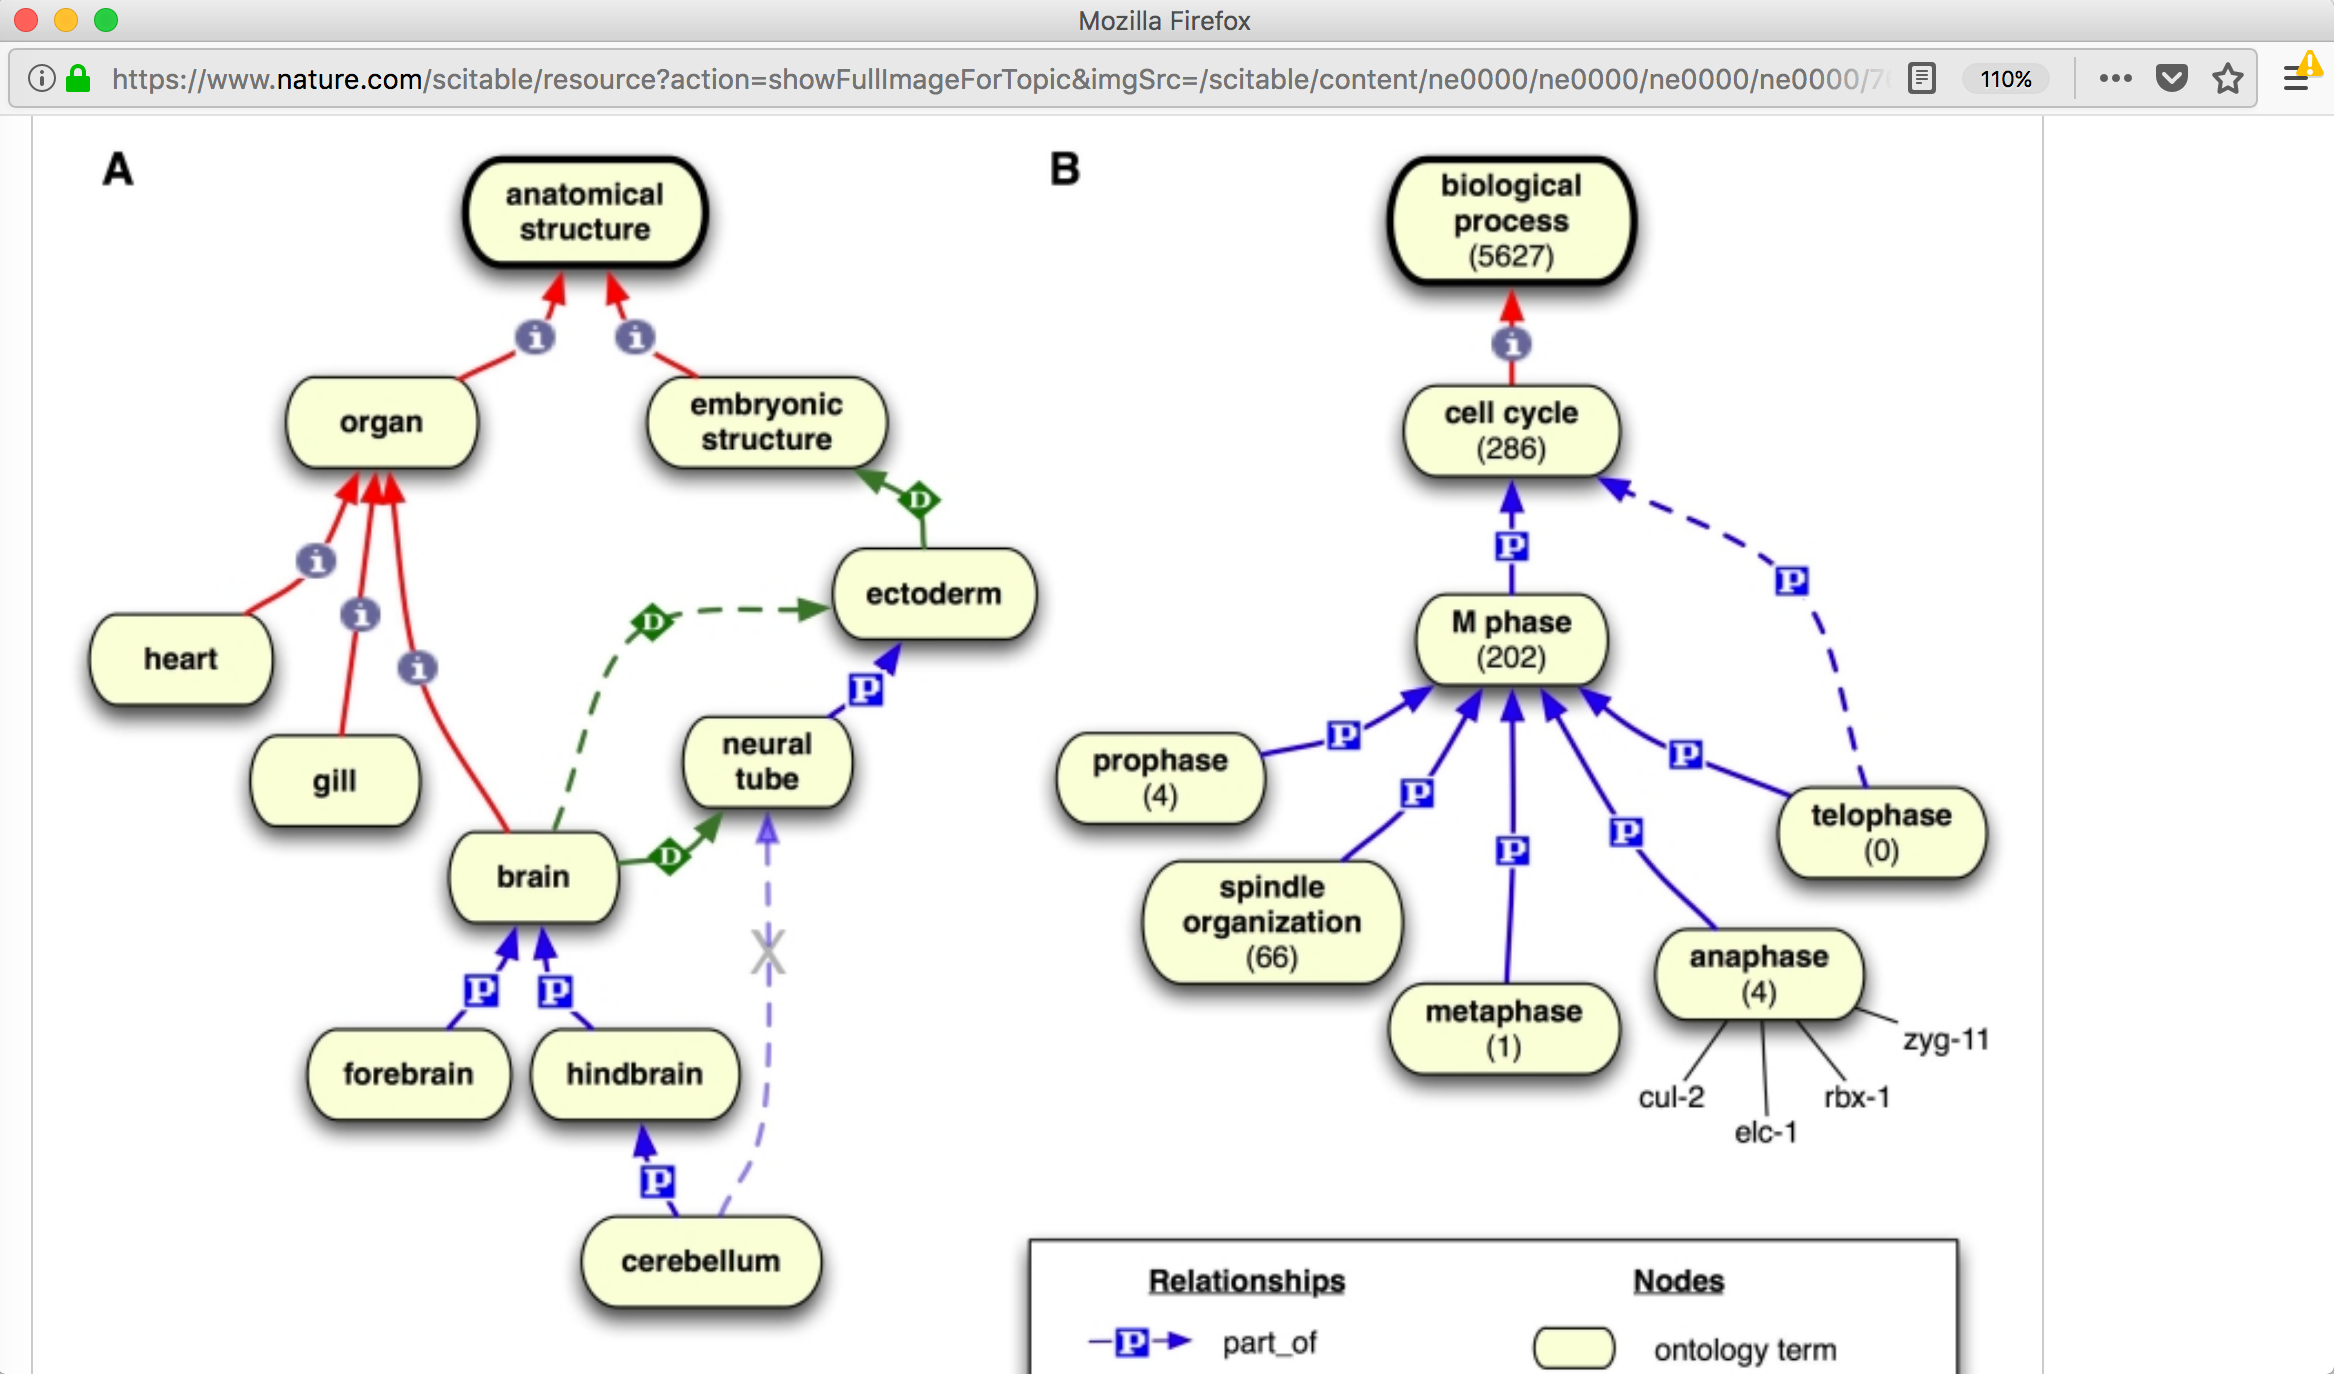
\includegraphics[width=1\textwidth]{example_ontology.png}
  \caption{Contoh sebuah ontology}
\end{figure}

\textit{Vocabulary} (dapat diartikan sebagai kosa kata baku dalam suatu RI) diperlukan untuk menyeragamkan terminologi/istilah yang dipakai dalam metadata. Sebagai contoh, saat kita memasukkan kata kunci "hidrologi", maka dokumen apa saja yang akan muncul karena terkait dengan kata kunci tersebut. Salah satu database vocabulary adalah \href{https://bartoc.org/en}{Burton}.

Metadata diperlukan untuk (\href{http://dspacecris.eurocris.org/bitstream/11366/29/1/PositionPaperRoadMap20100610.pdf}{State of the Art and Roadmap for Current Research Information Systems and Repositories}):

\item \textbf{Integritas}: suatu obyek dalam repositori hanya akan ada bila nilai ada pada metadatanya. Begitu pula sebaliknya, sebuah metadata adalah representasi keberadaan suatu obyek digital.

\item \textbf{Navigasi}: metadata adalah komponen penting yang dicari oleh mesin pencari. 

\item \textbf{Pengukuran (metric)}: pengukuran perlu dilakukan untuk mengetahui kinerja sistem. Proses ini memerlukan metadata. 

\end{enumerate}

%Referensi untuk dibaca: 

% RAND
% EMAST
% etc


\bibliographystyle{apalike-oadoi}
\bibliography{sample}

\end{document}